\section{Rappresentazione di dati e segnali}

    \subsection{Segnali semplici e composti}
    
        La funzione principale dello \textit{strato fisico} è trasportare i dati in forma di \textbf{segnali elettromagnetici} su un mezzo trasmissivo. Questo significa che, per essere trasmessi, i dati devono essere prima trasformati in segnali elettromagnetici.
        
        \vspace{3mm}
        
        \textbf{Esistono due tipi di dati: analogici e digitali.} I \textbf{dati analogici} sono informazioni (valori) rappresentate in forma continua (e cioè il cui dominio è un insieme infinito di possibili valori); invece, i \textbf{dati digitali} sono informazioni (valori) rappresentate in forma discreta (e cioè il cui dominio è un insieme finito di possibili valori, rappresentati con sequenze di 0 e 1).
        
        \vspace{3mm}
        
        \textbf{Esistono due tipi di segnali: analogici e digitali.} I \textbf{segnali analogici} possono assumere un infinito numero di valori in un dato intervallo; invece, i \textbf{segnali digitali} possono assumere solo un numero finito di valori in un dato intervallo.
        
        \begin{center}
            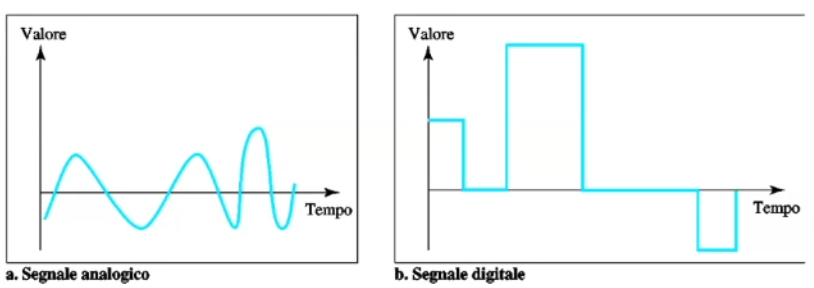
\includegraphics[scale=0.25]{images/Esempio-Segnali.png}
         \end{center}
        
        \vspace{3mm}
        
        Sia i segnali analogici che digitali possono assumere due forme: \textbf{periodica} (varia regolarmente nel tempo) e \textbf{aperiodica} (varia senza regolarità nel tempo).
        
        \vspace{3mm}
        
        In particolare, se un segnale digitale ha \(L\) livelli, ogni livello può facilmente rappresentare \(log_2 L\) bit. La lunghezza di tali bit è l'analogo della lunghezza d'onda per i segnali analogici. Può essere interpretata come la distanza (o lo spazio) che la rappresentazione di un bit occupa sul mezzo trasmissivo. E' funzione di velocità di propagazione e rappresentazione utilizzata. La lunghezza di 1 bit equivale a \((\text{velocità di propagazione})*(\text{durata di 1 bit})\).
        
        Osserviamo che il concetto di livello è escluso dei segnali digitali.
        
        \begin{center}
            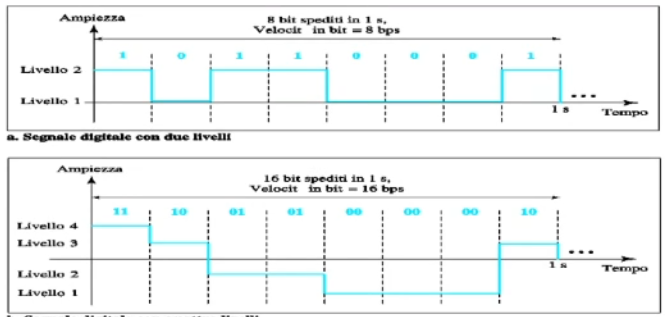
\includegraphics[scale=0.45]{images/Segnali-Digitali-Esempio.png}
        \end{center}
        
        \vspace{3mm}
        
        Per le reti di comunicazione, normalmente vengono usati segnali analogici periodici e segnali digitali non periodici. I primi richiedono minore larghezza di banda e possono essere semplici o composti. I secondi possono rappresentare facilmente i dati.
    
    \subsection{Descrizione delle onde sinusoidali dei segnali analogici}
    
        \subsubsection{Segnali analogici semplici}
    
            \textbf{Un segnale analogico è detto \textit{semplice} se non può essere decomposto in segnali più semplici}, e viene rappresentato graficamente con una curva oscillante (come la funzione \(sen\)). Tale curva dipesa dall'\textit{ampiezza massima} (o di picco; è il valore assoluto del segnale nella sua intensità massima - per segnali elettrici si misura in \textit{volt}), dalla \textit{frequenza} e dalla \textit{fase}.
            
            \vspace{3mm}
            
            Le onde semplici hanno molte applicazioni: ad esempio, sono adatte per il trasporto di energia elettrica, ma sono inadatte per il trasporto di segnali che rappresentano suoni, dati e quindi per le reti di comunicazione in generale.
            
            \vspace{3mm}
            
            Un segnale semplice è descritto tramite:
            
            \begin{itemize}
            
            \item 
                Il \textbf{periodo} è il tempo necessario affinché un segnale completi un ciclo, espresso in \textit{secondi}. Il ciclo è la porzione di curva che si ripete.
            
            \item
                La \textbf{frequenza} è il numero di periodi in 1 secondo, espresso in \textit{hertz}. Può essere interpretata come la velocità con cui il segnale cambia nel tempo, ed è direttamente legata alla velocità di trasmissione.
            
            \item
                Si osservi che il periodo è l'inverso della frequenza, e viceversa.
            
                \begin{center}
                    \(f=\frac{1}{T}\)
                    
                    \(T=\frac{1}{f}\)
                \end{center}
            
            \item
                La \textbf{fase} descrive la posizione dell'onda sinusoidale rispetto al tempo 0, espressa in \textit{gradi} o \textit{radianti}. Se si pensa all'onda come un qualcosa che può essere spostato avanti o indietro lungo l'asse del tempo, la fase descrive l'ampiezza di tale spostamento.
            
                \begin{center}
                    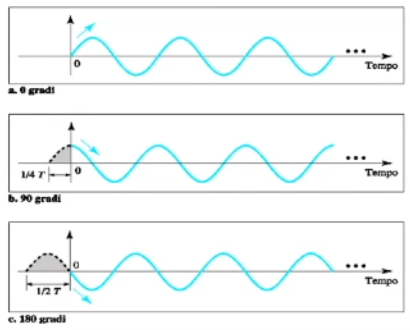
\includegraphics[scale=0.45]{images/Fase.png}
                \end{center}
            
            \item
                La \textbf{lunghezza dell'onda} mette in relazione il periodo \(T\) (o la frequenza \(f\)) con la velocità di propagazione \(c\) del segnale del mezzo. La lunghezza d'onda è funzione del mezzo di trasmissione (oltre che del segnale) e rappresenta la distanza (o meglio lo spazio) che un ciclo del segnale occupa sul mezzo trasmissivo, espressa in \textit{micron}.
            
                \begin{center}
                    \(\lambda=c*T=\frac{c}{f}\)
                \end{center}
            \end{itemize}
            
        \subsubsection{Segnali analogici composti}
        
            Parliamo adesso dei segnali analogici composti. \textbf{Le onde composte sono la somma di onde sinusoidali semplici.} L'\textit{analisi di Fourier} mostra che un qualsiasi segnale composto è la somma di onde semplici con diverse frequenza, ampiezze e fasi.
        
            Un segnale composto è descritto tramite:
            
            \begin{itemize}
                \item
                    Lo \textbf{spettro} è l'insieme delle frequenze di un segnale composto.
                
                \item
                    La \textbf{larghezza di banda} è la differenza fra la frequenza più alta e la più bassa nello spettro.
            \end{itemize}
    
    \subsection{Deterioramento del segnale}
    
        I segnali viaggiano lungo il mezzo trasmissivo, il quale causa un deterioramento del segnale: questo implica che il segnale ricevuto non è esattamente quello inviato. Le cause sono, in genere, l'attenuazione, la distorsione o il rumore del segnale.
        
        \subsubsection{Attenuazione}
        
            L'\textbf{attenuazione} è la perdita di energia subita quando il segnale, viaggiando lungo il mezzo trasmissivo, deve superare la resistenza del suddetto. Questo è anche il motivo per cui il filo elettrico si riscalda quando viene attraversato dal segnale: parte dell'energia elettrica, infatti, viene convertita in calore. 
            
            In termini pratici, man mano che il segnale viaggia si subisce una perdita di energia poiché il mezzo trasmissivo, per sua natura, è dotato di una resistenza che attenua il passaggio del segnale stesso, provocando un fenomeno di perdita di energia, per l'appunto - tale perdita di energia viene trasformata in calore, determinando il surriscaldamento del mezzo trasmissivo.
            
            La perdita di energia è espressa in decibel, che misurano la potenza \textit{relativa} di due segnali (o dello stesso segnale) in due punti differenti. 
            
            \(dB = 10*log_10 \frac{P_2}{P_1}\)
            
            Per ripristinare il valore corretto di decibel viene generalmente posto un \textit{amplificatore} nei pressi del nodo destinatario.
        
        \subsubsection{Distorsione}
        
            La \textbf{distorsione} è il cambiamento della forza del segnale, molto tipica dei segnali composti costituito da varie frequenze. Ogni componente (frequenza) del segnale ha una propria velocità di propagazione lungo il mezzo trasmissivo, il che causa un ritardo per l'arrivo della destinazione.
            
            In particolare, se guardiamo un segnale composto come un insieme di segnali semplici, allora successivamente al viaggio individuale di questi segnali lungo il mezzo trasmissivo, può risultare che il loro arrivo non sia sincronizzato, producendo un segnale composto finale diverso da quello desiderato. I segnali arrivano non allineati, ma risulta distorto, poiché non coincide con quello spedito.
        
        \subsubsection{Rumore}
        
            Il \textbf{rumore} è dovuto ad interferenze esterne. Può essere termico (causato dal movimento casuale degli elettroni nel mezzo trasmissivo), indotto (causato da sorgenti come motori o altri dispositivi esterni), ad impulsi (causato da fonti esterne come fulmini, che causano un repentino cambio del segnale) o ad interferenze (causato dall'eccessiva vicinanza fra due cavi che trasmettono segnali).
    
    \subsection{Velocità di trasferimento}
    
        Per trovare il limite teorico alla velocità in bit occorre conoscere il rapporto fra la potenza del segnale e la potenza del rumore del canale. Ricordiamo che il mezzo trasmissivo, per sua natura, è dotato di rumore.
    
        \begin{center}
            \(SNR[Signal-toNoise-Ratio] = \frac{potenza\ \ segnale}{potenza\ \ rumore}\)
            
            \vspace{3mm}
            
            \(SNR_{db} = 10 log_{10} SNR\)
        \end{center}
        
        La velocità di trasferimento dei bit dipesa dalla larghezza di banda, dal numero di livelli del segnale e dalla qualità del canale (che induce o meno al rumore). I due risultati teorici per il calcolo della velocità massima su un canale di comunicazione sono forniti dal \textit{Teorema di Nyquist} e dal \textit{Teorema di Shannon}.
        
        I teoremi di Shannon e Nyquist forniscono due risultati in letteratura estremamente validi per ciò che concerne la velocità idealistica ed effettiva della trasmissione di dati.
        
        \subsubsection{Teorema di Nyquist}
        
            \(\text{velocità in bit per secondo}=2*(\text{larghezza di banda})*log_2 L\)
            
            \vspace{3mm}
            
            Questo ideale risultato parte dal presupposto che un canale non sia condizionato dal rumore.
            
            \(L\) è il numero di livelli del segnale che possono essere utilizzati per rappresentare i dati. Aumentando \(L\) si aumenta la velocità. Questo risultato ornisce la velocità teorica massima alla quale possiamo spedire i dati. Chiaramente, non si può aumentare \(L\) a piacere, poiché - da un punto di vista pratica - si ridurrebbe l'affidabilità della trasmissione, aumentendo la probabilità di riscontrare errori: questo perchè, all'aumentare della capienza del canale, è più probabile commettere errori.
        
        \subsubsection{Teorema di Shannon}
        
            \(\text{capacità}=(\text{larghezza di banda})*log_2 (1+SNR)\)
            
            \vspace{3mm}
            
            \textbf{Nella realtà non esistono canali senza rumore}. Questo teorema fornisce un valido risultato teorico per la capacità (cioè la velocità massima) di un canale in \textit{bps}. Il risultato è in funzione del canale di trasmissione col suo rumore (SNR) e non dei livelli dei canali.
            
            Poiché Shannon considera l'SNR, considera automaticamente anche il rumore del canale.
            
        Nelle applicazioni pratiche, si sfruttano ambo i teoremi. Shannon determina la capacità (cioè la velocità di trasferimento massima), mentre Nyquist determina il numero di livelli necessari per ottenere la velocità massima. Significa utilizzare la formula inversa di Nyquist per ottenere \(L\), che è un risultato pratico molto valido.
            
    \subsection{Prestazioni della rete}    
        
        Per misurare l'efficienza di una rete, in genere, si valutano numerosi parametri. Definiamo le più importanti.
        
        \subsubsection{Larghezza di banda}
        
            Espressa in \textit{hertz}, è la larghezza di banda delle frequenze utilizzate per la trasmissione. E' dunque l'intervallo di frequenze utilizzate dal segnale, o l'insieme di frequenze che possono essere spedite lungo il canale.
            
            Espressa in \textit{bps}, misura la velocità massima alla quale possiamo spedire bit sul canale.
            
        \subsubsection{Throughput}
        
            \textbf{Misura quando velocemente possiamo spedire i dati su una rete.} A differenza della larghezza di banda, è una \textbf{misura effettiva}.
            
        \subsubsection{Latenza}
        
            \textbf{Misura quanto tempo occorre a trasferire un intero messaggio.} In effetti, è il tempo misurato dal primo bit spedito  all'ultimo bit arrivato, e consiste in tempo di trasmissione, di propagazione, di attesa e di inoltro.
            
            \vspace{3mm}
            
            Il tempo di trasmissione misura il tempo per immettere i dati sul mezzo.
            
            \begin{center}
                \(T_T = \frac{\text{dimensione dei dati (in bit)}}{\text{larghezza di banda}}\)
            \end{center}
            
            Il tempo di propagazione misura il tempo necessario al segnale per propagarsi sul mezzo trasmissivo.
            
            \begin{center}
                \(T_P = \frac{\text{distanza}}{\text{velocita' di propagazione del segnale}}\)
            \end{center}
            
            I tempi di attesa e di inoltro riguardano, rispettivamente, l'attesa nei nodi intermedi e il tempo necessario al nodo intermedio per smistare il messaggio.
            
        \subsubsection{Prodotto banda-ritardo}
        
            E' il prodotto \(\text{(larghezza di banda)}*\text{(latenza)}\).
            
            Definisce il numero di bit che servono per riempire il canale.
            
            In termini informali, il prodotto banda-ritardo rappresenta il numero di bit si possono avere lungo il mezzo trasmissivo prima che il primo bit arrivi a destinazione.
            
        \subsubsection{Jitter}
        
            Misura la variabilità del ritardo con cui vari messaggi, cioè i pacchetti, vengono consegnati alla destinazione. E' chiaramente necessario che i pacchetti vengano consegnati con lo stesso ritardo.